\documentclass[journal,twoside]{IEEEtran}
\usepackage{cite}
\ifCLASSINFOpdf
   \usepackage[pdftex]{graphicx}
\else
   \usepackage[dvips]{graphicx}
\fi
\usepackage{url}
\usepackage[utf8]{inputenc}
\usepackage{amssymb}
\usepackage{amsmath}
\usepackage[caption=false]{subfig}
\DeclareMathOperator*{\argmax}{argmax}
% correct bad hyphenation here
\hyphenation{op-tical net-works semi-conduc-tor}
\pagenumbering{gobble}
\setcounter{page}{0}

\begin{document}

\title{Deep Reinforcement Learning in Distributed Optimization}
\author{Marcus~Lindström and Jahangir~Jazayeri}

\markboth{C4: Distributed optimization}%
{C4: Distributed optimization} 
\maketitle

% As a general rule, do not put math, special symbols or citations
% in the abstract or keywords.
\begin{abstract}
	
Reinforcement learning has recently become a promising area of machine learning with significant achievements in the subject.
Recent successes include surpassing human experts on Atari games and also AlphaGo becoming the first computer ranked on the highest professional level in the game Go, to mention a few.\par
This project aims to apply Policy Gradient Methods (PGM) in a multi agent environment. PGM are widely regarded as being applicable to more problems than for instance Deep Q-Learning but have a tendency to converge upon local optimums. In this report we aim to explore if an optimal policy is achievable with PGM in a multi-agent framework.\par
Numerical simulations implementing the aforementioned method in an environment with up to 4 agents and moving obstacles showed a convergence and the efficiency of the approach. A relatively small amount of collisions took place once the learnt agents were tested. These result differed when changing some parameters such as learning rates and number of neurons in the neural network.\par
The conclusion was that a very fast convergence upon at least a local optimal policy was achieved in this setting.
\end{abstract}

\section{Introduction}

In the late 1950's, ``Machine Learning" was coined as a field that is concerned with the study of
algorithms that learn from data and make predictions. While the subject suffered periods
of low interest (primarily during the 70’s), it has now seen an increase in popularity much due to deep learning methods becoming feasible.

Google’s DeepMind team caused lots of media attention when their AlphaGo AI won against
the reigning world champion go player\cite{website123}, and has since further developed this into Alpha Go Zero; an AI based on “Tabula Rasa” learning. Meaning it learns without any human
intervention or data, but exclusively from self play to the point where it wins in about 90\%\cite{silver} of games against the earlier champion beating version.

This report investigates methods for solving a specific problem
within a paradigm of machine learning called Reinforcement Learning (RL), an area defined by the problem of how AI's ought to make actions within an environment in order to maximize
cumulative reward. The problem that we address in this report consists of implementing model free deep learning algorithms
for optimizing the cooperative behavior of multiple agents. Our special case of this consist of a $\mathbb{R}^2$ grid in which agents move along common paths, having knowledge of other agents absolute positions and speeds while transporting items between unique sets of starting and ending positions.

\section{Preliminaries and background} \label{prelback}

This section covers our approach to finding an optimal control policy in the case of multi agent reinforcement learning (MARL). First we outline the theory and methodology needed for finding solutions in the case of single agents. Then move on to how these can be manipulated and combined with \textit{deep learning} algorithms for tackling the more general case. 

\subsection{Single agent reinforcement learning}

Definition 1 below introduces the finite Markov decision process (MDP) which is the formal model used in single agent RL:\\

\noindent\textbf{Definition 1.} \textit{A finite Markov decision process is a tuple $\langle\mathcal{S,A},T,R,\gamma\rangle$ where $\mathcal{S}$ is the finite set of environment states, $\mathcal{A}$ is the finite set of agent actions, $T:\mathcal{S}\times\mathcal{A}\times\mathcal{S}\rightarrow [0,1]$ is the state transition probability function, $R:\mathcal{S}\times\mathcal{A}\times\mathcal{S}\rightarrow\mathbb{R}$ is the reward function, and $\gamma$ is a discount factor $\gamma\in [0,1]$.}\\

For deterministic systems, the transition function is replaced and takes on another form: $\bar{T}:\mathcal{S}\times\mathcal{A}\rightarrow\mathcal{S}$, meaning also that the reward function is determined completely by the current action and state. 

At each time step $t$ the environment is described by $s_t\in\mathcal{S}$, the agent observes the state and takes an action $a_t\in\mathcal{A}$ which transitions the state to $s_{t+1}$ with probability $T(s_{t+1}\mid s_t, a_t)$. The transition is evaluated by the reward $r_{t+1}\in\mathbb{R}$ according to $r_{t+1}=R(s_{t+1}\mid s_t,a_t)$.

The agent follows a policy $\pi(s):\mathcal{S}\rightarrow\mathcal{A}$, i.e., a mapping from perceived environment states to actions, and the goal is suitably to find the optimal policy $\pi^*$ which maximizes its total expected reward, this is where the learning of the agent takes place, from modifying $\pi$ over time. By taking the above into consideration we introduce the \textit{state value function for policy $\pi$}\cite{Sutton:1998:IRL:551283}: 

\begin{equation}
v_\pi(s)=\mathbb{E}_\pi \Bigg[\sum_{k=0}^{\infty}\gamma^{k}r_{t+k+1}\Bigg\vert s_t = s\Bigg], \forall s\in\mathcal{S},
\end{equation}

\noindent which describes for each state $s$ its value for the agent to start in if following policy $\pi$ (the use of the discount factor $\gamma$ can be interpreted as minding less about future reward). The optimal value function $v^*(s)$ is closely related to the optimal policy $\pi^*$, and as can be seen in equation \eqref{eq:2a} and \eqref{eq:2b}, finding $v^*(s)$ means finding $\pi^*(s)$:

\begin{subequations}
\begin{align}
v^*(s)&=\max_{\pi}v_\pi(s)=v_{\pi^*}(s), \label{eq:2a}\\
\pi^*(s)& = \argmax_{a\in\mathcal{A}}\sum_{s'\in\mathcal{S}}T(s'\mid s,a)v^*(s'). \label{eq:2b}
\end{align}
\end{subequations}

The aforementioned theory has so far not exclusively been revolving around model free RL per se, but it does apply to it. In the case of having complete knowledge of the MDP, one can actually find the optimal control policy without ever letting an agent ``step into" the environment with use of planning algorithms. The RL problem is not so simple, instead the agent does not know beforehand how the environment will change in response to its actions or how much reward it's going to get. Instead, the agent has to learn from experience and adapt to its environment by taking actions within it and observing the consecutive states it ends up in. 


\subsection{Neural networks}

Deep learning methods are based on using \textit{neural networks} in order to find (or learn) a set of weights that characterize the importance of different attributes of data. In the case of RL, these weights are used in order for the agent to make 'good' decisions and thus defines the policy described in section \ref{prelback}.

A neural network consists of artificial neurons that maps input to an output, mimicking the biological ones in the human brain. Consider the simplest case of one neuron taking as input for example, $X_1$, $X_2$ and $X_3$  see figure \ref{singleneuron}. 

\begin{figure}[!h]
	\centering
	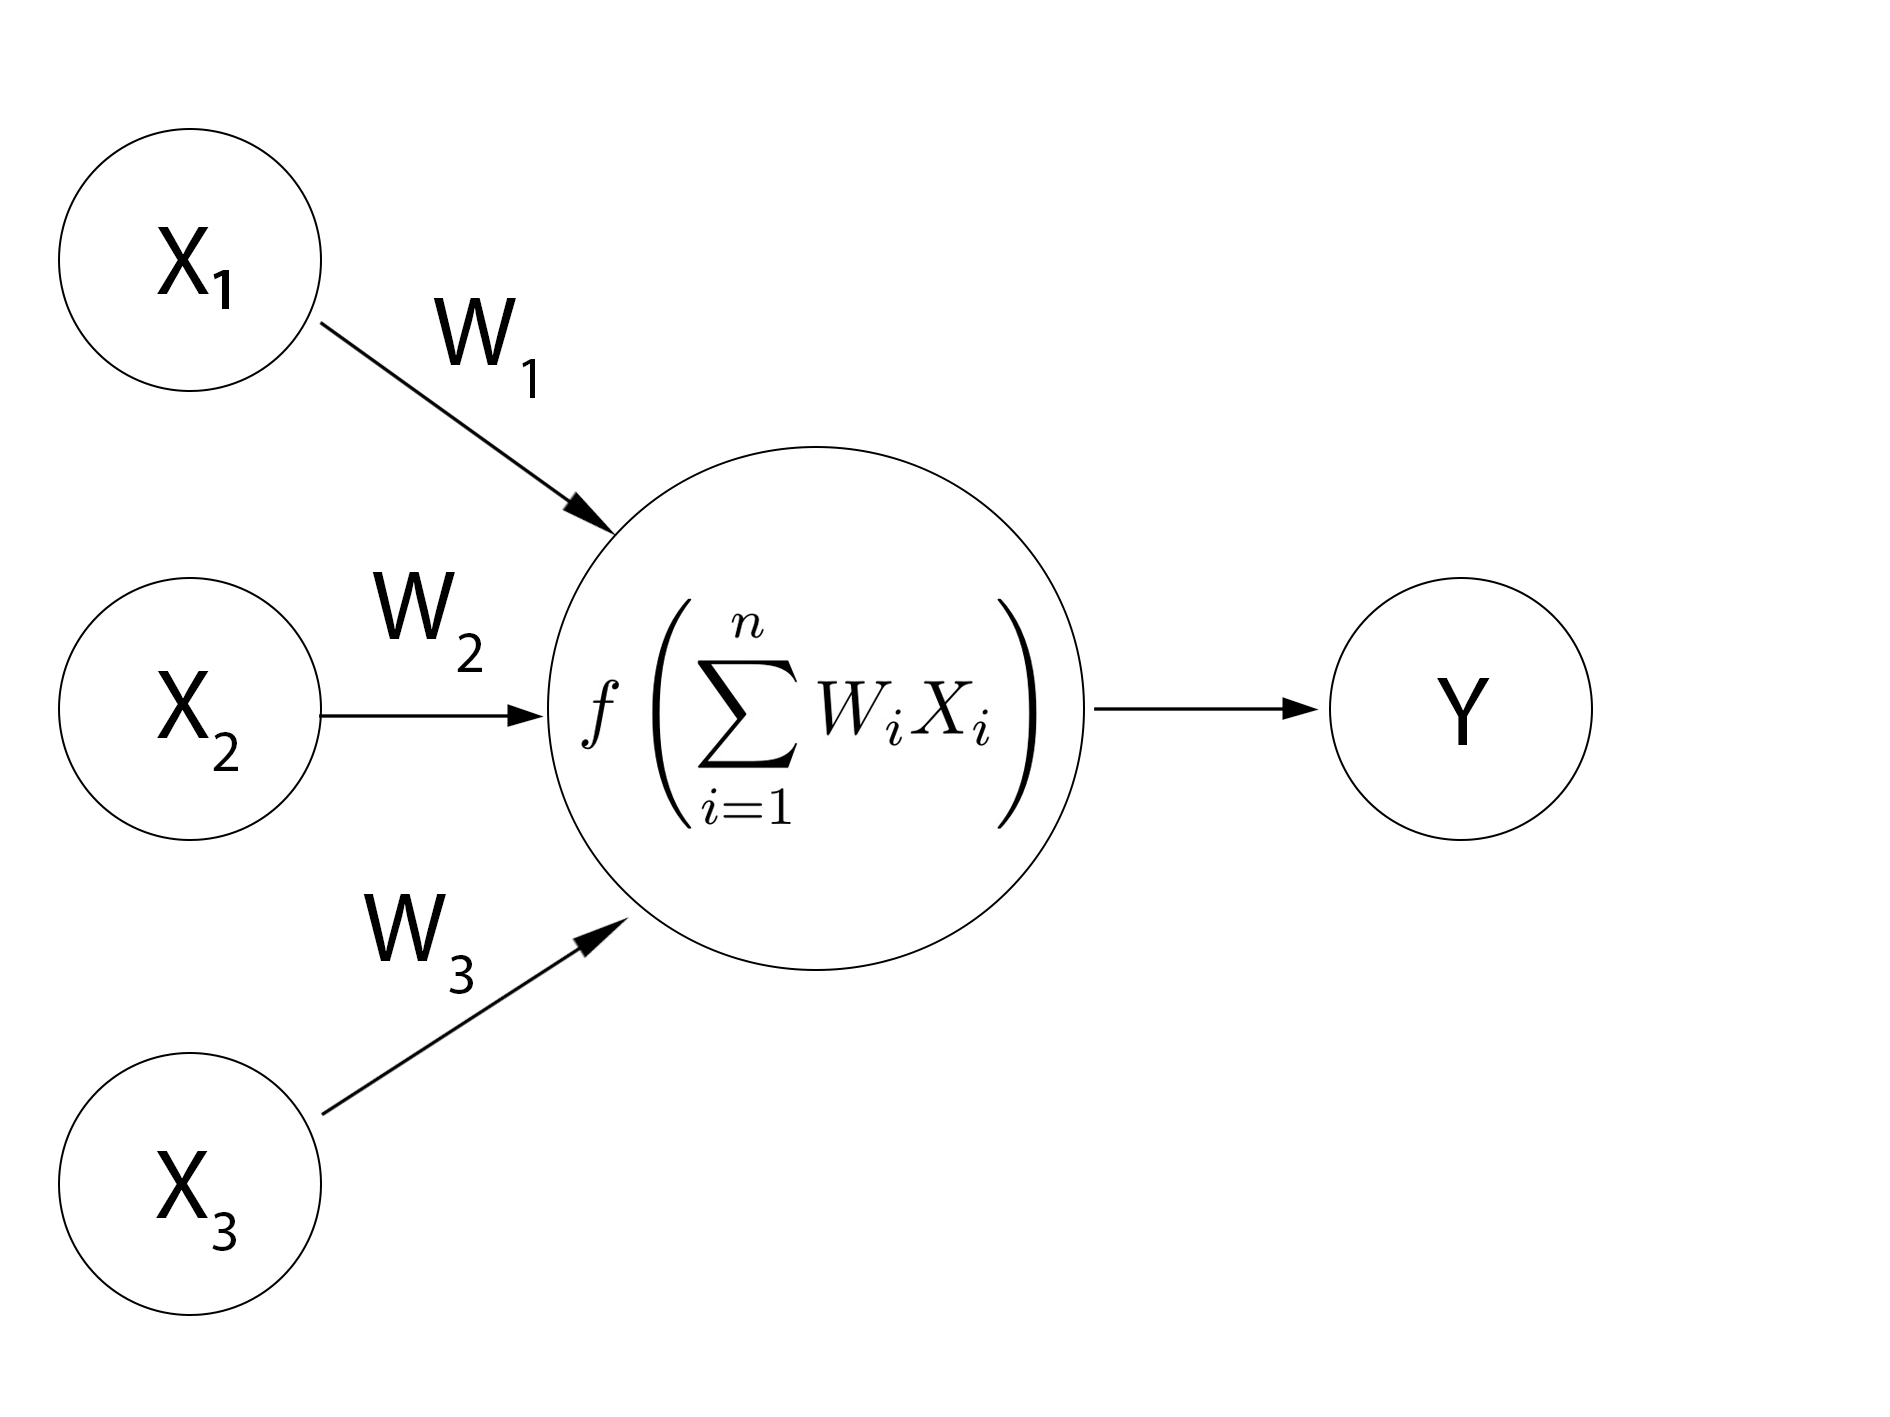
\includegraphics[width=0.8\columnwidth]{network}
	\caption{Illustration of a single neuron taking three inputs and mapping them to a single output through an activation function $f$.}
	\label{singleneuron}
\end{figure} 

The weight $W_i$ can be thought of as the importance of attribute $X_i$ for said neuron. The activation function denoted $f: \mathbb{R}\mapsto\mathbb{R}$ takes as input the sum of all weights times the attributes and maps this to an output, it can be modeled differently depending on the scenario but a few worth mentioning are the \textit{sigmoid}, \textit{tanh} and \textit{rectified linear} functions given in descending order by equations \eqref{eq:3a}, \eqref{eq:3b} and \eqref{eq:3c} below and visualized in figure \ref{actfunc}.


\begin{subequations}
	\begin{align}
	f(z)&=\frac{1}{1+e^{-z}}, \label{eq:3a}\\
	f(z)&=\frac{e^{z}-e^{-z}}{e^{z}+e^{-z}}, \label{eq:3b}\\
	f(z)&=\max(0,z). \label{eq:3c}
	\end{align}
\end{subequations}

\begin{figure}[!h]
	\centering
	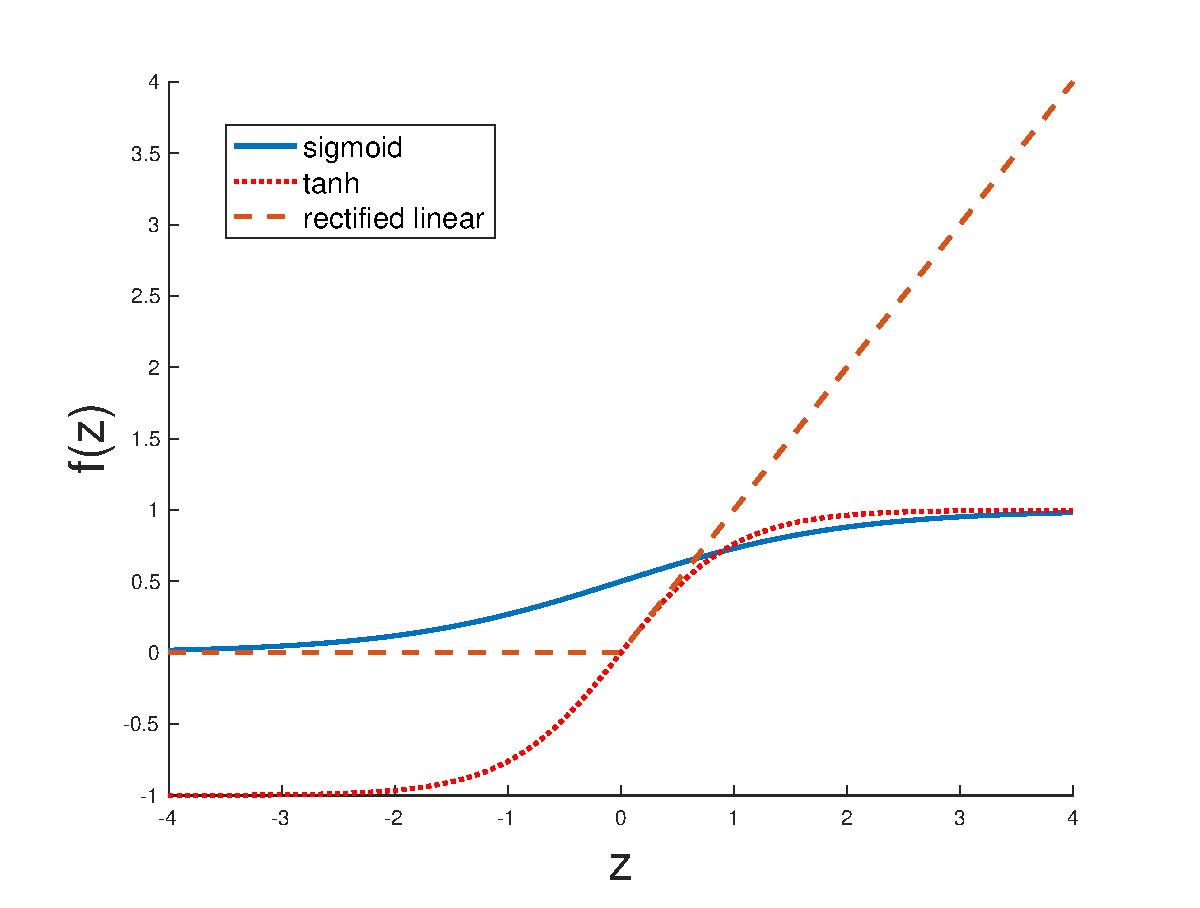
\includegraphics[width=0.9\columnwidth]{Activation_functions}
	\caption{Different types of activation functions used in neural networks.}
	\label{actfunc}
\end{figure}

\begin{figure}[!h]
	\centering
	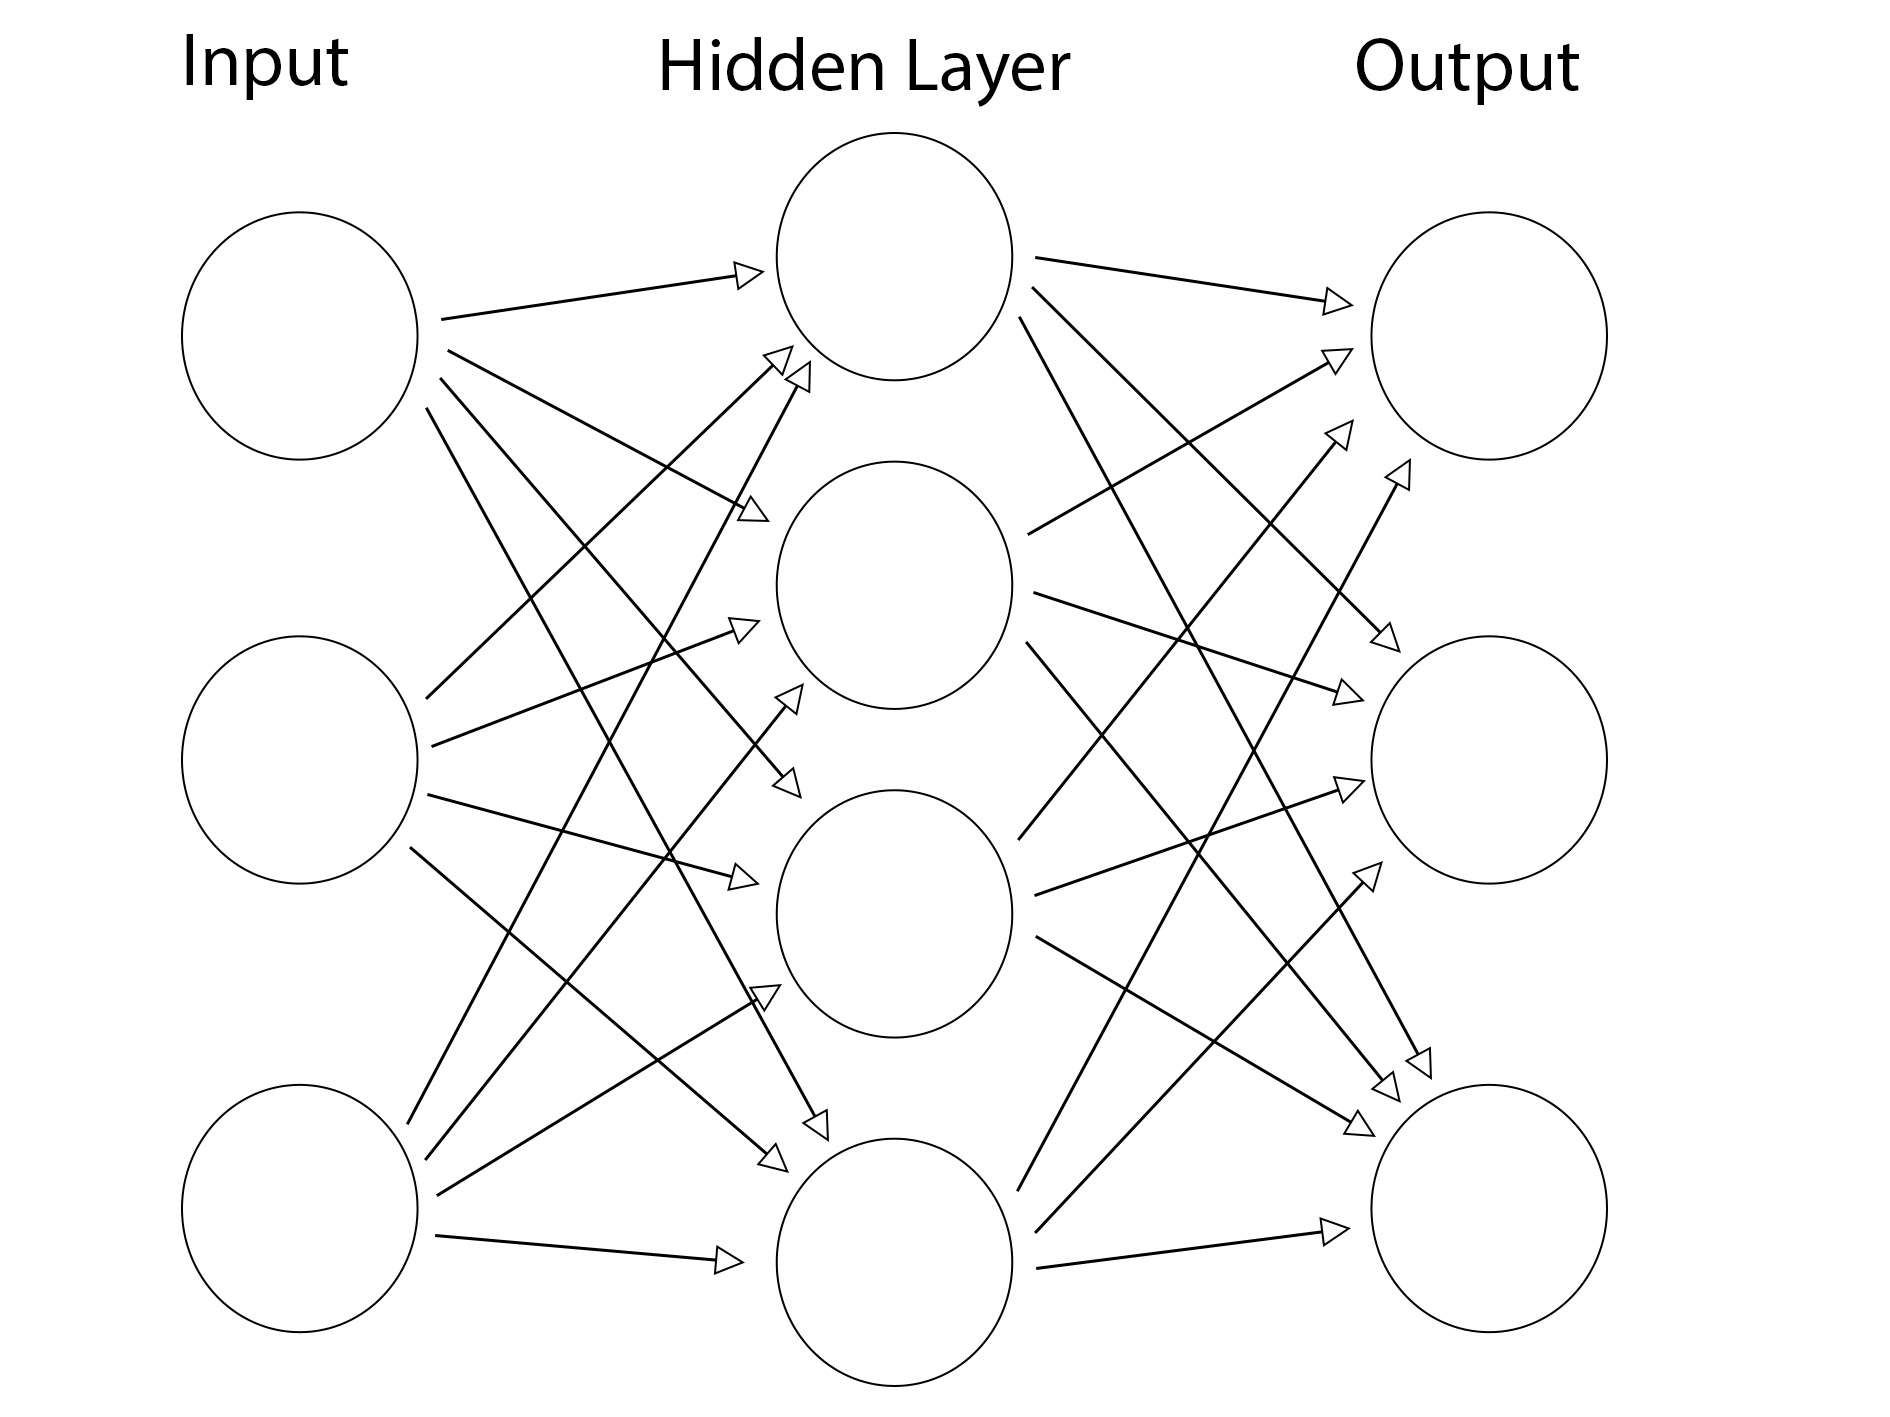
\includegraphics[width=0.9\columnwidth]{figure-1}
	\caption{A neural network with one hidden layer.}
	\label{nnonelayer}
\end{figure}

A more complex network comprises many connected neurons in different layers where one neurons output may be the input of another, see figure \ref{nnonelayer}. From the outside, only the input and output layers are observed thus the middle layer is referred to as 'hidden' and an arbitrary amount of these may be used. If we denote the amount of layers by $\eta_l$, which is equal to three in our case, and denote layer $l$ by $L_l$ we can collect the weights in matrices $W^{l}$ where element $W_{(ij)}^{l}$ corresponds to the weight connecting neuron $i$ in layer $l$ with neuron $j$ in layer $l+1$. Furthermore, let $a_{i}^{l}$ denote the output of neuron $i$ in layer $l$, and $z_{i}^{l}$ the sum of weighted inputs to neuron $i$ in layer $l$, (for $l=1$ we simply let $a_{i}^{1} = x_i$ where the $x_i$'s are the input values to the network). Also note that when modeling a neural network, one can use varying kinds of activation functions for each layer, thus we let the activation function for layer $l$ be denoted $f_l$.

The output of our example network is referred to as a hypothesis $h_W(x)$ and with the terminology laid out above we can describe our networks computations with the following equations, (we let the activation function $f_l$ take vectors as inputs and compute element-wise outputs):

\begin{subequations}
\begin{align}
a^{(1)}&=x,\\
z^{(2)}&=W^{(1)}a^{(1)},\\
a^{(2)}&=f_2(z^{(2)}),\\
z^{(3)}&=W^{(2)}a^{(2)},\\
h_W(x)&=a^{(3)}=f_3(z^{(3)}).
\end{align}
\end{subequations}

There are other kinds of architectures for building neural networks which we will not cover here, our example network is referred to as \textit{Feedforward}, characterized by connections between neurons not forming cycles or loops.

Initially the weights $W^{l}_{ij}$ are chosen randomly, otherwise it would result in $a^{(2)}_1=a^{(2)}_2=a^{(2)}_3$... etc. because of symmetry. To update them smart, an algorithm called Gradient Descent can be utilized which lightly speaking means that one follows the opposite direction of a loss function $J(W)$'s (indicating how 'bad' an output is), gradient with respect to the weights according to the following:

\begin{equation}
\label{5}
W^{l}_{ij} = W^{l}_{ij}-\alpha\frac{\partial}{\partial W^{l}_{ij}}J(W).
\end{equation}

The partial derivatives $\frac{\partial}{\partial W^{l}_{ij}}J(W)$ are calculated numerically with help of a method called \textit{Backpropagation} \cite{BP} and $\alpha$ is chosen as to indicate how sensitive each update of the network should be to the gradient. Note that the loss function is not restricted to being convex which means the algorithm is susceptible to converging upon local optima rather than global ones, this is in practice though usually not an issue. 

\subsection{Deep reinforcement learning}

In order to utilize neural networks when optimizing a control policy for a reinforcement agent one can use different approaches. One example is to approximate the value function mentioned earlier which indirectly gives the policy, in this paper though we use a direct optimal policy approximation through what are referred to as \textit{Policy Gradient Methods}. The network takes as input a representation of the state and directly maps it onto a probability distribution of actions (or a policy), this is then used in order to determine what action to take. 

The loss function introduced in the previous part has to be modeled in such a way so as to represent how actions and rewards are related, a positive reward has to be the result of a good action. We introduce the \textit{Cross Entropy} function $J(W)$:

\begin{equation}
J(W)=-\sum rlog\pi(a\mid s;W).
\end{equation}

We see that in order to minimize $J(W)$, the policy has to favor actions that give positive reward given a certain state.

\section{Methods}

In this section, we discuss the practical issues of our implementation. We show also how the rewards affected each agent with respect to what state it transitioned to after taking an action. Furthermore, we represent how the environment was defined and represented.

\subsection{Environment and rewards}

The environment consisted of a 10 by 10 grid with three horizontally moving obstacles where each agent had its own respective goal (see figure 4). The rewards were adjusted so that the agents always received a small negative reward from each transition. Moreover, a larger penalty from either taking an action that puts it on top of another agent or obstacle and a big positive reward from getting to its goal (see table 1).

The state representation that the environment supplied agents with consisted of a tuple with components representing relative distances and directions to obstacles, agents and its own goal and also rewards from each. It also contained information regarding what direction each moving obstacle was headed.

\begin{figure}[!h]
	\centering
	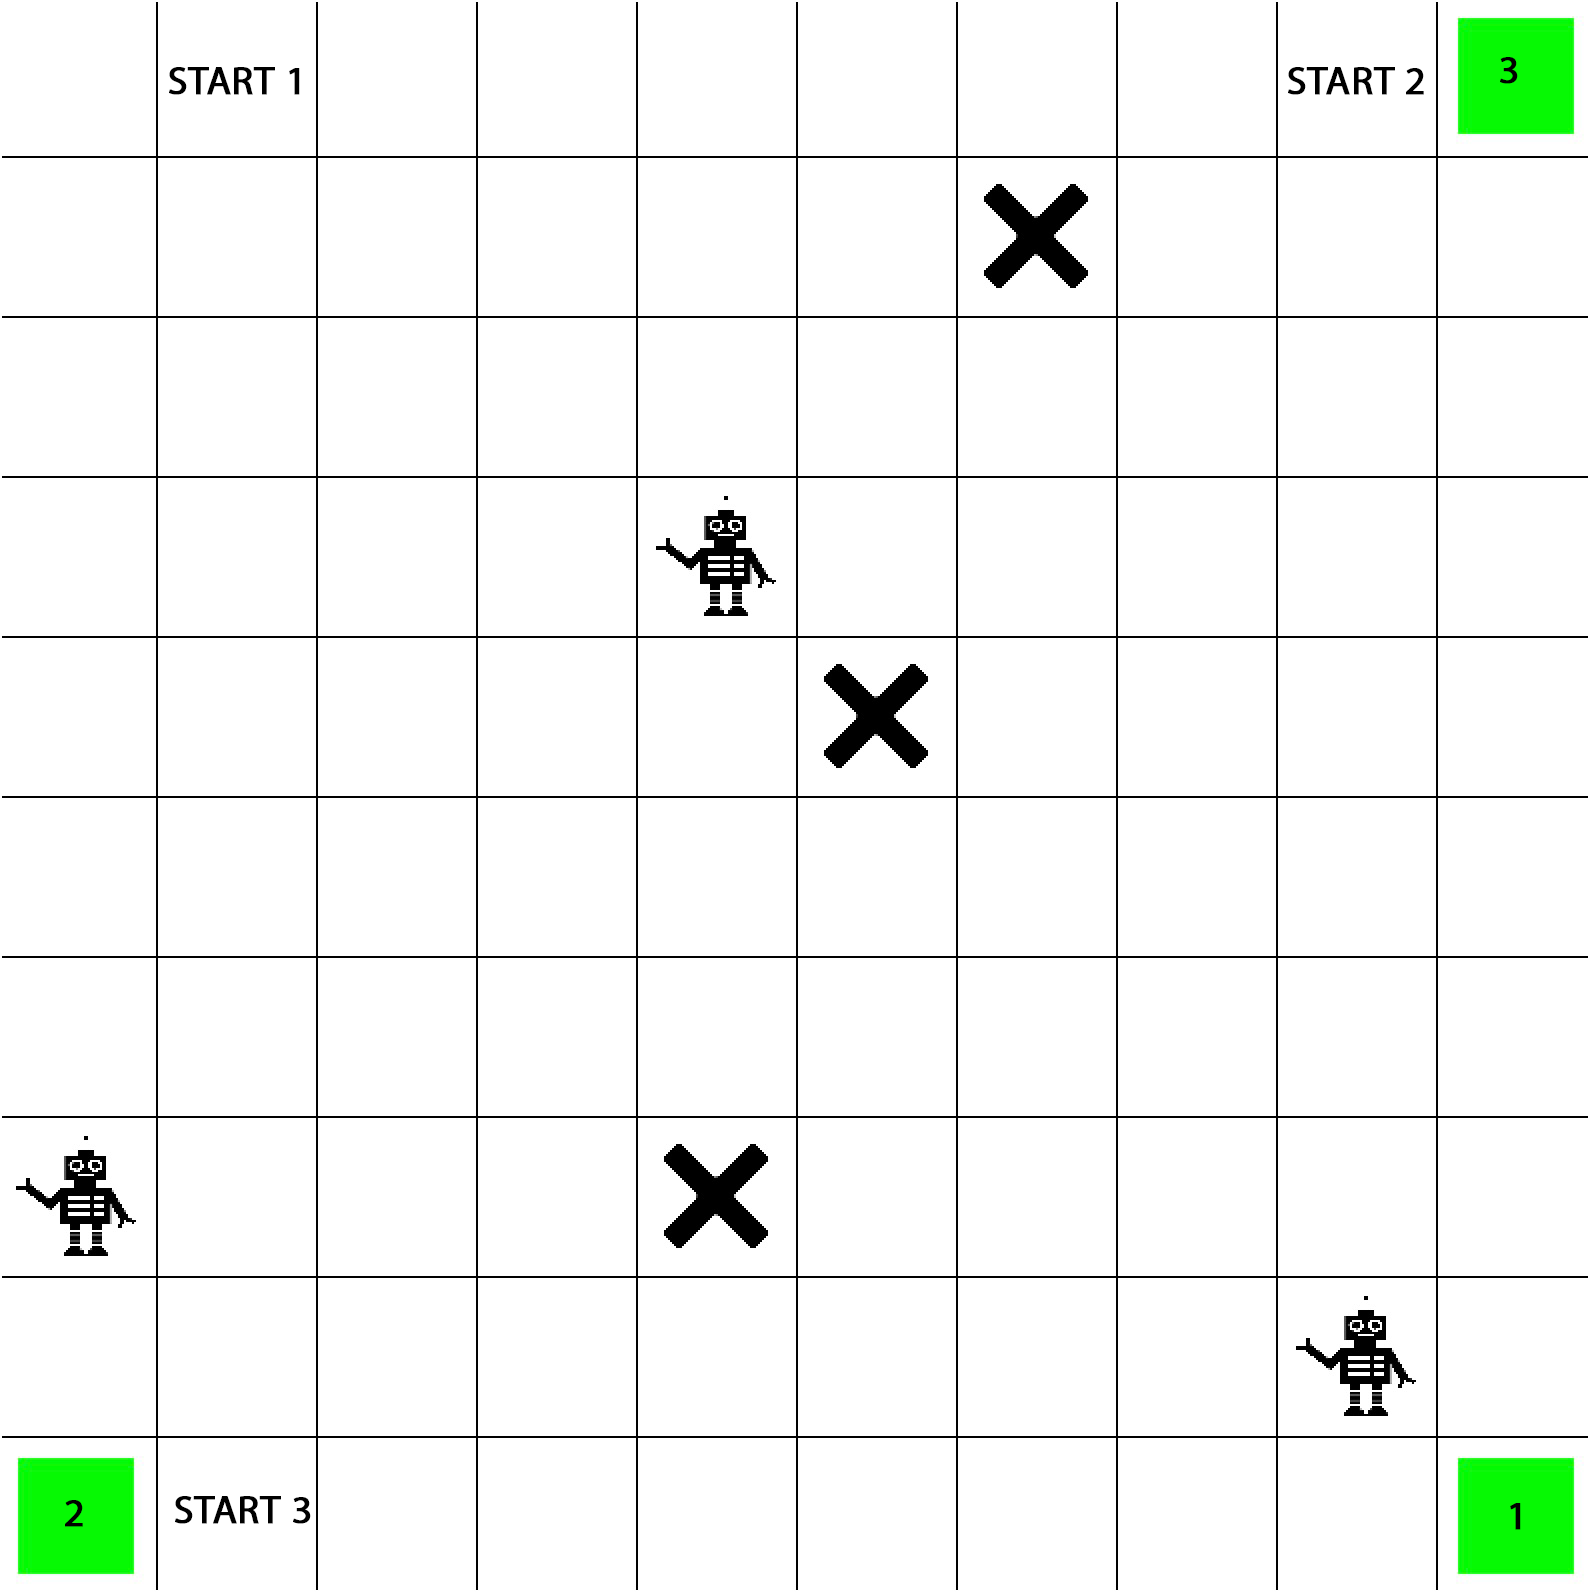
\includegraphics[width=0.9\columnwidth]{Grid}
	\caption{The visualized environment with three agents in it, crosses represent horizontally moving obstacles and squares are stationary goals.}
	\label{fig_sim}
\end{figure}

\begin{table}[h!]
	\begin{center}
		\caption{Distribution of rewards that agents could receive from taking an action that transitions it to a different state.}
		\label{tab:table1}
		\begin{tabular}{l|r}
			\textbf{State} & \textbf{Reward} \\
			\hline
			Obstacle & -1\\
			Another agent & -1\\
			Goal & 2\\
			All states & -0.1\\
		\end{tabular}
	\end{center}
\end{table}

\subsection{Algorithm details}

Initially, the goals, agents and obstacles were placed at preset locations. This was followed by the obstacles updating their position with one step horizontally and only changing direction if encountering a wall. All agents could then take one step and in response the obstacles took another and so on. If one agent was to find its way to goal it froze in place until all other agents also found theirs thus ending one episode. 

All the implementations were done in \textit{Python3} using an edited version of a publicly available \textit{GitHub} code \cite{code}.

\newpage

\section{Main Results}


\begin{figure}[!h]
	\centering
	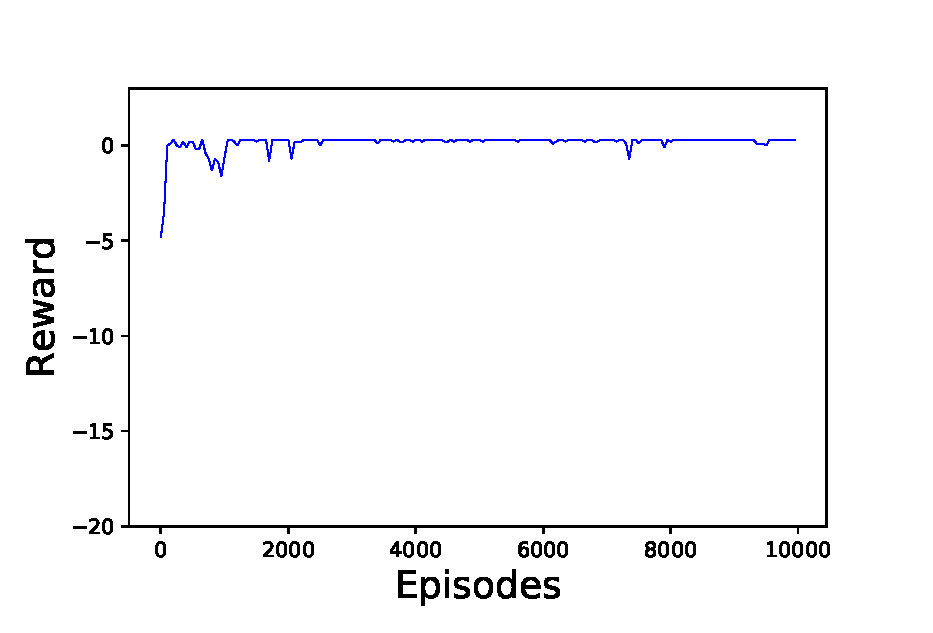
\includegraphics[width=\columnwidth]{1Agent_24n__2l_180000steps_110s}
	\caption{Results from 2500 episodes one agent, two hidden layer with 24 neurons. The maximum reward was 0.3.}
	\label{1agent24n}
\end{figure}

\begin{figure}[!h]
	\centering
	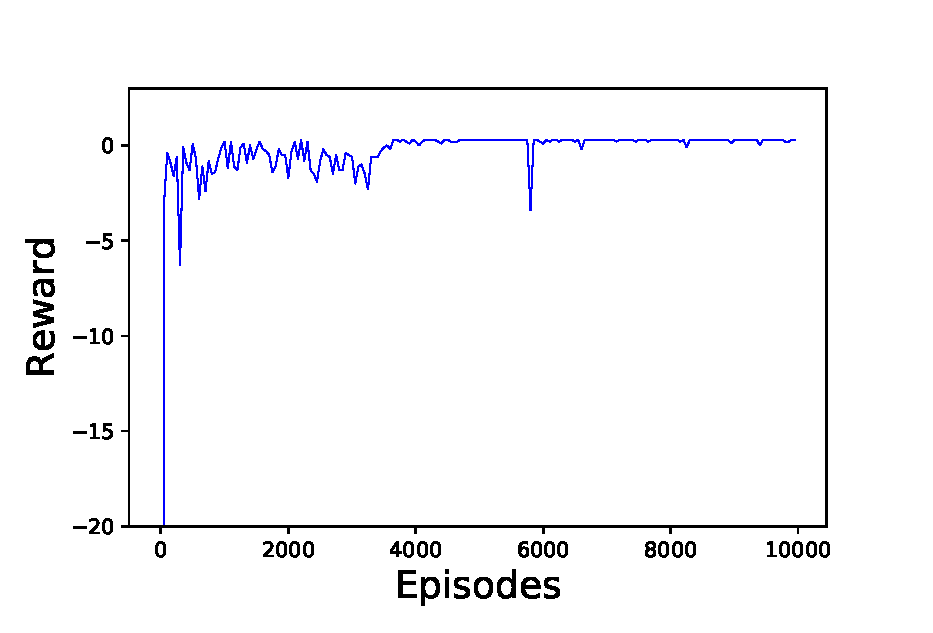
\includegraphics[width=\columnwidth]{1Agent_32n__2l_215000steps_125s}
	\caption{Results from 2500 episodes one agent, two hidden layer with 24 neurons. The maximum reward was 0.3.}
	\label{1agent32n}
\end{figure}

\begin{figure}[!h]
	\centering
	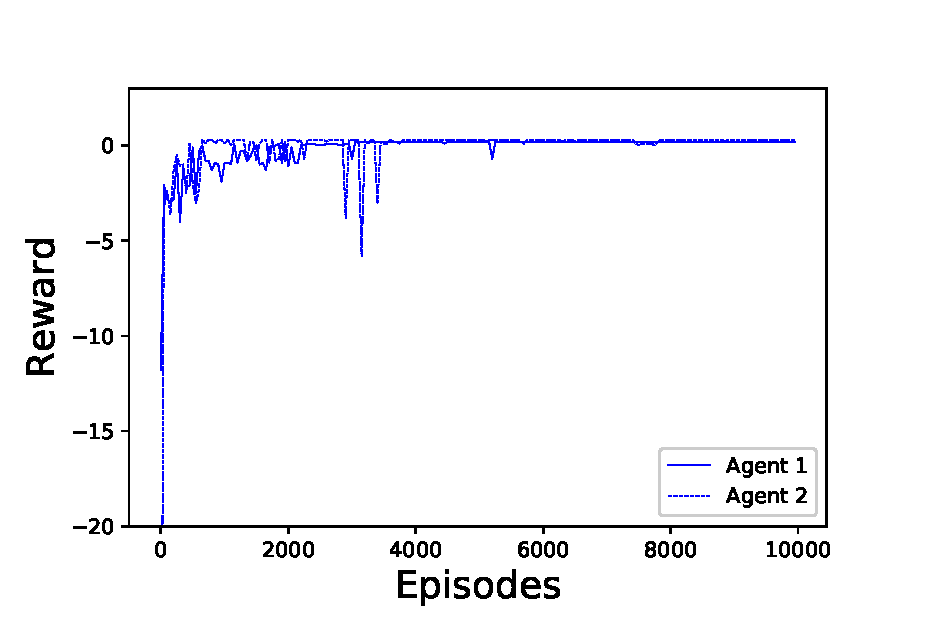
\includegraphics[width=\columnwidth]{2Agent_24n_2l_380000steps_251s}
	\caption{Results from 2500 episodes two agents, two hidden layer with 24 neurons. The maximum reward for the agents were [0.2, 0.3].}
	\label{2agent24n}    
\end{figure}

\begin{figure}[!h]
	\centering
	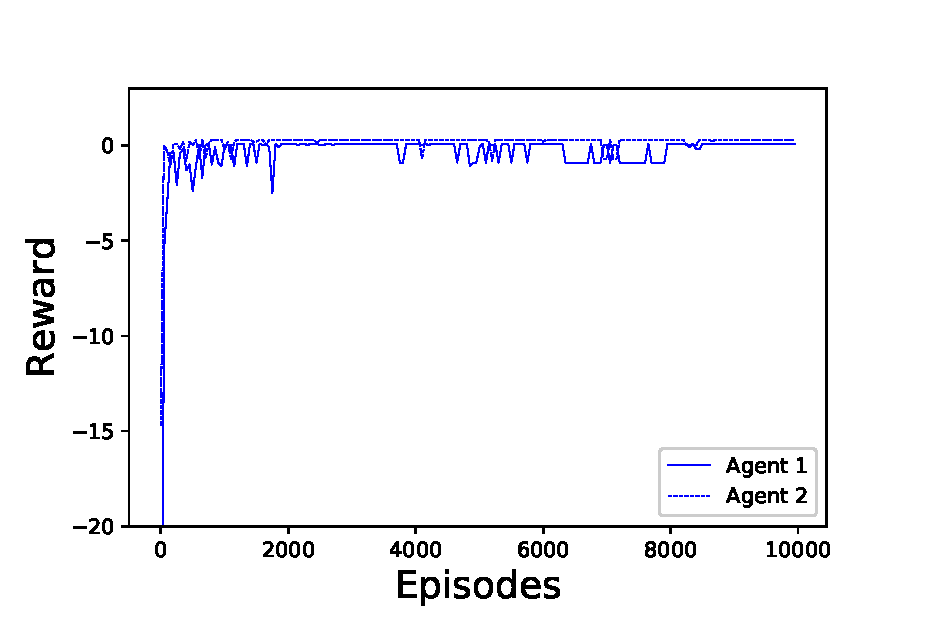
\includegraphics[width=\columnwidth]{2Agent_32n_2l_380000steps_250s}
	\caption{Results from 2500 episodes two agents, two hidden layer with 32 neurons. The maximum reward for the agents were [0.2, 0.3].}
	\label{2agent32n}    
\end{figure}

\begin{figure}[!h]
	\centering
	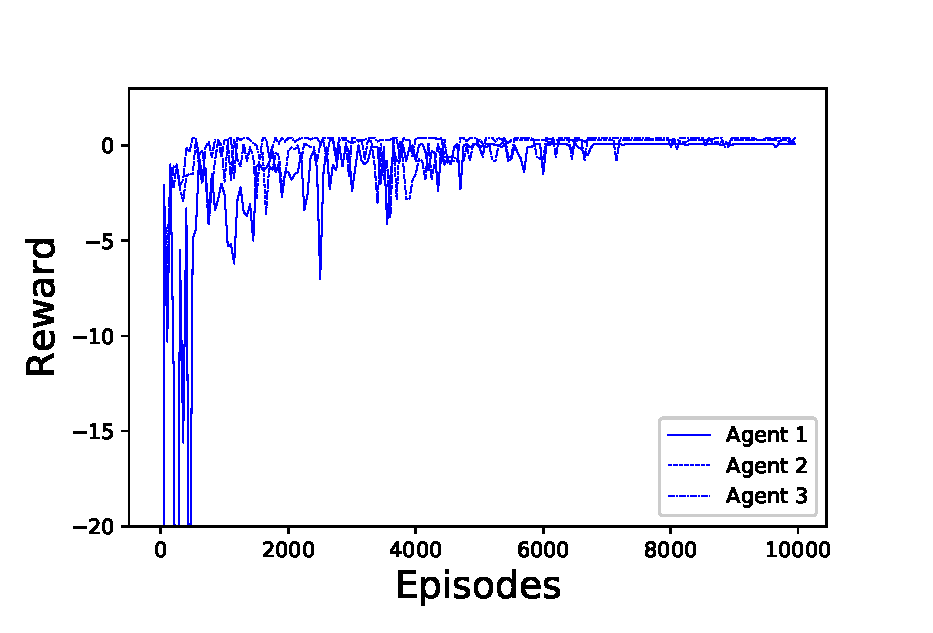
\includegraphics[width=\columnwidth]{3Agent_32n_2l_737343}
	\caption{Results from 2500 episodes thee agents, two hidden layer with 32 neurons. The maximum reward for the agents were [0.2, 0.3, 0.4].}
	\label{3agent32n}    
\end{figure}

\begin{figure}[!h]
	\centering
	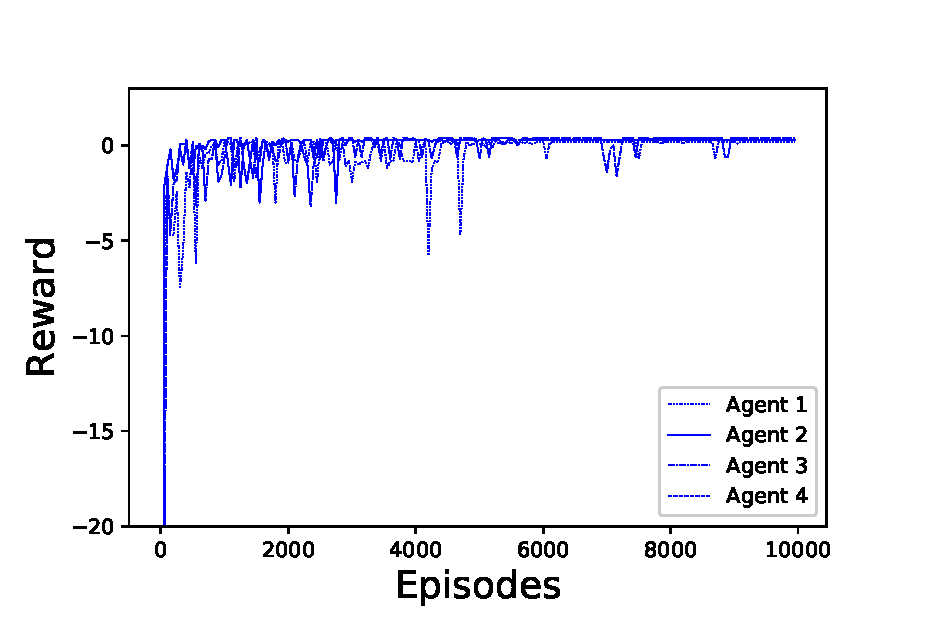
\includegraphics[width=\columnwidth]{4Agent_32n_784243steps}
	\caption{Results from 2500 episodes four agents, two hidden layer with 32 neurons. The maximum reward for the agents were [0.2, 0.3, 0.4, 0.4].}
	\label{4agent32n}    
\end{figure}

\clearpage

\begin{table}[!h]
	\centering
	\caption{Average performance/computational time for a learning sequence of one to four agents.}
	\label{perf}
	\begin{tabular}{crrrrr}
		\hline
		\textbf{No Agents / nodes} & \textbf{Global steps} & \textbf{Time (s) }
		\\ \hline
		1 / 24            & 180,000       & 110       \\ 
		1 / 32            & 180,000       & 125       \\ 
		2 / 24            & 380,000      & 250       \\ 
		2 / 32            & 390,000     & 260      \\ 
		3 / 32            & 730,000     & 390    \\ 
		4 / 32            & 900,000      & 500     \\ 
	\end{tabular}
\end{table}

\begin{table}[!h]
	\centering
	\caption{Average number of collisions per 2000 episodes evaluated over ten runs with learned policies.}
	\label{perf}
	\begin{tabular}{rrrrrr}
		\hline
		\textbf{No. agents}    & \textbf{Obstacle collisions} & \textbf{Agent collisions} \\ \hline
		1            & 0       & -       \\ 
		2            & 1.4       & 0       \\ 
		3            & 10.1      & 0.1       \\ 
		4            & 23.7      & 4.4      \\ 
	\end{tabular}
\end{table}

%\newpage

\section{Discussion}
This section covers a direct analysis of the results given in the previous section along with concerns regarding generality and modeling of our algorithm. We also set the stage for possible future research on the subject.

\subsection{Data Analysis}
All of the measurements performed and the data gathered for the results were computed on a desktop with 4 cores, 2,2 GHz CPU and 16GB of RAM. The different times and performance measurements are with regards to that computational power. During this section of the report references to certain terms will be made, we begin with describing these. An episode means that all of the agent have reached their respective goals and a learning sequence is defined as completing 10000 episodes.

\subsection{Learning sequences}

Table \ref{perf} functions as an quick overview for the time spent on a learning sequence. The nodes defined in the table corresponds to the number of neural network nodes in the two hidden layers. Global steps represents the number of actions taken by all agents and the time was clocked from start to finish. The values of Table \ref{perf} are not from a single learning sequence but are instead composed of rounded averaged values from three sessions. \par
Fig. \ref{1agent24n} until \ref{4agent32n} shows the gathered results of a complete learning sequence. They are portrayed by graphs of rewards as a function of episode. The interval for all six figures have been set to be x-axis $ = [0, 10^{4}] $ and y-axis $ = [-20, 3] $. In all of the figures discussed here there have been large negative rewards especially during the first episodes that were not able to fit. \par
When increasing the number of agents to three or above the acquired policy could often lead to a special situation. The majority of the agents converged upon a reward near their respective maximum. The remaining agents would instead choose a policy leading to a negative reward caused for example by a collision. This behavior is partly a consequence of the reward design in the algorithm. In MARL the  design of a suitable reward signal is a central problem and we used a local one based on individual behavior which is prone to educate selfish agents. They ignore the others needs in order to maximize their own reward and leaves them in a more difficult state \cite{Reward}. A typical scenario in the learning sequence can look as in figure \ref{selfish} where it is clear that when one agent chooses greedily others may suffer.
\begin{figure}[!h]
	\centering
	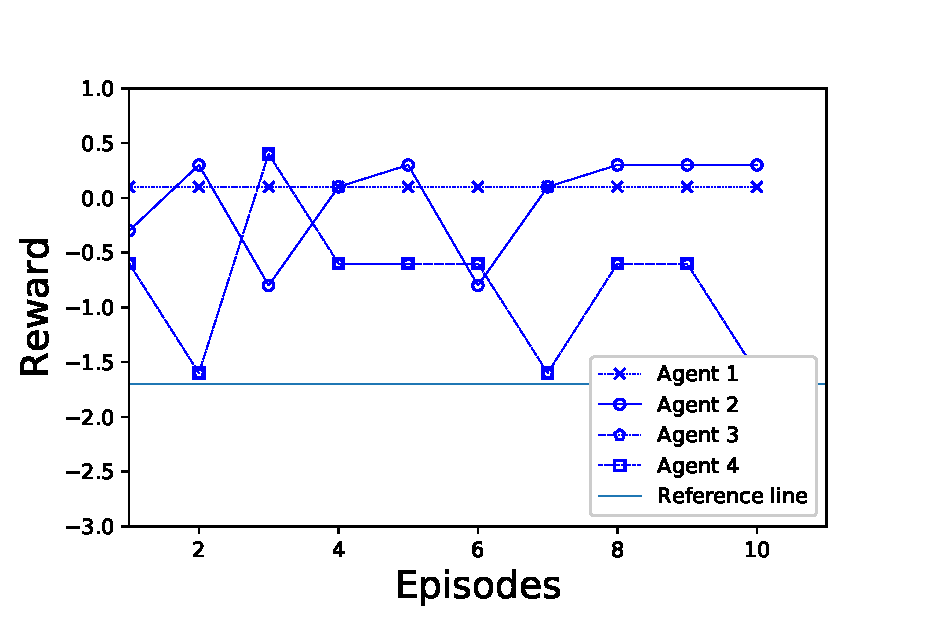
\includegraphics[width=\columnwidth]{selfish}
	\caption{Four agent environment, the reference line is at -1.7 on the reward axis and corresponds to the agents going the fastest way to goal with two collisions on the way.}
	\label{selfish}    
\end{figure}

\subsection{Evaluation of Learned Policies}

After having learned policies over the course of 20.000 episodes, these were evaluated based on their collision frequencies presented in table 3. A collision is defined as one agent taking an action that puts it on top of either an obstacle or another agent, therefore; agents who stand still and collide do not constitute a collision. 

Not surprisingly, we see an increase in the number of collisions when more agents are being used, although not substantial. These numbers could likely be lowered with help of more learning and fine tuning of $\alpha$ (see eq. \eqref{5}). 

When visualizing the system, it is apparent that these policies constitute agents moving along paths with as much space between them as possible, thus lowering the chance of having agents collide. This as opposed to making more room between agents and obstacles, the reason being likely that the behaviors of these are easier to learn since their movements are deterministic.
 
\subsection{Generality and Model Analysis}

This project used the direct approach of attempting to map states to actions i.e. Policy Gradient Methods. As has been touched upon in the report, the method is susceptible to converging upon local optima rather than global ones. This was noticed as the agents sometimes would stay at certain positions and not continue to explore the grid. However, if an agent was to find its goal, it did not take much time for it to afterwards find its optimal policy, though not necessarily after having explored the whole environment. 

The learned policies do seem to generalize in upscaled environments but fail to be meaningful in different settings, i.e. repositioning of goals and starting positions. This however does not have to be a problem depending on the situation in which the algorithm were to be implemented.

\subsection{Future Work}

\begin{itemize}
\item A rather large bias that was introduced in our algorithm was how the network output was used in order to take actions, this could have been modeled differently e.g. instead taking its argmax and using an \textit{epsilon greedy}\cite{epsilon} approach.  

\item It would be interesting to compare convergence rates between our approach and others, e.g. \textit{deep Q-value netwoks}\cite{Qlearn}.

\item Learned policies in less complex environments e.g. with less agents could be utilized in order to learn more complex policies.

\item Since the problem has a direct graphical interpretation, an approach using \textit{Deep Convolutional Neural Networks} \cite{Conv} would be worth inspecting. 

\item Modeling the environment with more bias towards making collisions more frequent e.g. choke points could be worth exploring to evaluate behavior of a more cooperative nature.

\item In this project a constant learning rate was used to generate policies, taking into account that this parameter has a big impact on the result; it would be wise to consider ways to choose this with more care, e.g. a decaying scheme.

\item Implementing a mixed reward signal i.e. a combination of a local and global one, e.g. methods mentioned in \cite{Reward}. This could be compared to the approach considered in this report. 

\end{itemize}

\section{Conclusions}

\begin{itemize}
	\item Finding optimal policies for multi agent systems does work up to a limited amount of agents when using policy gradient methods. Depending on the nature and complexity of the system, simplifications may have to be made.
	\item The initial neural network weights do affect the convergence rate greatly when networks are learning. 
	\item Learned policies are sensitive to how rewards are defined during learning, if chosen poorly; unwanted behavior does arise in the result.
	\item Learned policies do not generalize to new environments, though they may be utilized in similar settings to make the learning more effective.
	\item The learning rate i.e. $\alpha$ is hard to choose so as to not end up in a local maximum but still find the optimal policy.
	
\end{itemize}

\section*{Acknowledgment}

The authors would like to thank Alexandros Nikou, Mina Ferizbegovic and Takuya Iwaki for their excellent feedback and help with organizing our work.

\ifCLASSOPTIONcaptionsoff
  \newpage
\fi

\bibliographystyle{IEEEtran}

\bibliography{./KEX_bib_example}

\end{document}